\documentclass[a4paper,11pt,twocolumn]{article}
%\documentclass[twocolumn,aps,pre,groupedaddress]{revtex4-1}

\usepackage{amsmath}
\usepackage{graphicx}
\usepackage{amsmath}
\usepackage{graphicx}
\usepackage{subfig}
\usepackage{epstopdf}
\usepackage{amssymb}

\begin{document}
\title{Non-parametric casual inference in bivariate time series data}
\author{James M. McCracken}
%\email{jmccrac1@masonlive.gmu.edu}
%\affiliation{School of Physics, Astronomy, and Computational Sciences \\ George Mason University \\ 4400 University Drive MS 3F3, Fairfax,VA. 22030-4444}
\author{Robert S. Weigel}
%\email{rweigel@gmu.edu}
%\affiliation{School of Physics, Astronomy, and Computational Sciences \\ George Mason University \\ 4400 University Drive MS 3F3, Fairfax,VA. 22030-4444}
\date{\today}

\begin{abstract}
...TBD...
\end{abstract}

%\pacs{}
\maketitle

\section{Introduction}
Casual inference in time series analysis centers on finding ``driving'' relationships between different time series data sets.  Showing the existence, rather than the exact nature, of the ``driving'' relationship between the sets is often the primary goal.  Thus, words like ``driving'', ``causality'', and related terms usually do not have straightforward analogs to the same terms used in other fields \cite{Granger1980,liu2012,Roberts1985}, e.g.\ , theoretical quantum or classical mechanics.  The development and study of such causal inference techniques is often called {\em time series causality}.  Most of these techniques fall into four broad categories, those related to transfer entropy \cite{Schreiber2000}, those related to Granger causality \cite{granger1969}, those related to state space reconstruction (SSR) techniques \cite{Sugihara2012}, and those related to lagged cross-correlation \cite{box2013,pascual2014}.  These techniques have found application in a wide range of fields including neuroscience (e.g.\ \cite{Kaminski2001}), economics (e.g.\ \cite{dufour1998,dufour2006}), climatology (e.g.\ \cite{mosedale2006}), and others.  

In this article, we introduce another time series causality technique derived directly from the definition of probabilistic causality \cite{}.  The new technique is then applied to synthetic and empirical time series data sets with known, or intuitive, causal structure.  We will discuss the strengths and weaknesses of the technique and try to frame how the technique may be useful for causal inference with empirical data.  Formal relationships to the other well known time series causality techniques, such as Granger causality or transfer entropy, will be the subject of future work.

\section{Causal Penchant}
Define the {\em causal penchant} as
\begin{equation}
\label{eq:pen}
\rho_{EC} := P\left(E|C\right) - P\left(E|\bar{C}\right)\;\;.
\end{equation}
The motivation for this expression is in te interpretation of $\rho_{EC}$ as a causal indicator; i.e.\ if $C$ causes (or {\em drives}) $E$, then $\rho_{EC} > 0$, and if $\rho_{EC} \le 0$, then the direction of causal influence in the system is undetermined.  If the effect $E$ is assumed to be recorded in one time series and the cause $C$ is assumed to be recorded in a different time series, then the direction of causal influence in the system can be determined by comparing various penchants calculated using both time series.  

The penchant definition includes the probability of an assumed effect occurring given a lack of the assumed cause,i.e.\ $P(E|\bar{C})$.  It may be argued that the lack of an assumed cause is unobservable, and thus, the penchant definition is not practically useful.  Pearl, and others, argue that causality depends on intervention, which implies the occurrence probability of the assumed effect should be conditioned on performing or not performing an action rather than on the presence or lack of an assumed cause \cite{Pearl}.  Bunge defines a causal relation as ``a relation among events'' \cite{Bunge}, again implying the lack of an assumed cause cannot be used to find causal relations.  These issues have been a part of probabilistic definitions of causality at least since the 1960s \cite{Suppes}, and we will not attempt to solve them in this article.  Our goal is the define a practical tool for causal inference.  As such, we will circumvent these philosophical issues in the definition of the penchant by deriving an expression that removes any conditioning on a lack of the assumed cause.

Eqn.\ \ref{eq:pen} can be rewritten using the law of total probability, i.e
\begin{equation}
\label{eq:totp}
P(E) = P(E|C)P(C) + P(E|\bar{C})P(\bar{C})\;\;,
\end{equation}
or Bayes theorem, i.e.\ 
\begin{equation}
\label{eq:bayes}
P(E|\bar{C}) = P(\bar{C}|E)\frac{P(E)}{P(\bar{C})}\;\;.
\end{equation}
The definition of probability complements implies $P(\bar{C}) = 1-P(C)$ and $P(\bar{C}|E) = 1-P(C|E)$.  Applying Eqn.\ \ref{eq:bayes} leads to
\begin{eqnarray*}
P(\bar{C}|E) &=& 1-P(C|E)\\
&=& 1-P(E|C)\frac{P(C)}{P(E)}
\end{eqnarray*}
Thus,
\begin{eqnarray*}
P(E|\bar{C}) &=& P(\bar{C}|E)\frac{P(E)}{P(\bar{C})}\\
&=&\left(1-P(E|C)\frac{P(C)}{P(E)}\right)\frac{P(E)}{1-P(C)}\;\;,
\end{eqnarray*}
and the second term in Eqn.\ \ref{eq:pen} has been written in terms of the of the first term.  This expression implies a penchant calculation containing only the conditional probability that is directly observed from the data, i.e.\
\begin{equation}
\label{eq:pencal}
\rho_{EC} = P(E|C)\left(1+\frac{P(C)}{1-P(C)}\right)-\frac{P(E)}{1-P(C)}
\end{equation}
This same expression can be derived without Eqn.\ \ref{eq:bayes} by using Eqn.\ \ref{eq:totp} to make the appropriate substitution for $P(E|\bar{C})$ into Eqn.\ \ref{eq:pen}.  This penchant calculation requires only a single conditional probability be estimated from the data.

The use of either Eqn.\ \ref{eq:totp} or Eqn.\ \ref{eq:bayes} may eliminate the concern that $P(E|\bar{C})$ is fundamentally unobservable.  It may also, however, introduce new philosophical concerns in the definition of the penchant.  For example, there has been no discussion of confounding.  Assuming, e.g.\  $P(\bar{C})=1-P(C)$ where $P(C)$ can be estimated from the data alone may be seen as an oversimplification of the dynamics generating the time series data; i.e.\ it may be seen as an assumption that the assumed effect is only caused by the assumed cause.  Thus, it may be argued that the penchant is an indication of predictability rather than causality (similar to arguments made regarding Granger causality \cite{Sugihara}).  These concerns will not be addressed directly in this article.  We emphasize, however, that we use terms like cause, effect, causal inference, and related terms to specifically refer to the expressions presented in this article and not to the general, or intuitive, meanings these terms are given elsewhere.

Assuming $P(E)$ and $P(C)$ can be estimated from the data alone is a key part of the penchant definition.  The penchant is non-parametric in the sense that there is no assumed functional relationship between the times series being investigated.  It will be shown below that the penchant is, essentially, a structured method for counting the data and using the those counts, along with notions from probabilistic causality, to infer which time series in a given pair might be seen as ``driving'' the other.  Motivation for the penchant is the need for a times series causality tool that relies only on the data.  It is often impossible to design experiments, or control interventions into the dynamics as discussed above, for many systems of interest, and it may be difficult to determine functional relationships between the time series data sets.

It follows from Eqn.\ \ref{eq:pen} that
\begin{equation}
\rho_{EC}\in\left[1,-1\right]\;\;,
\end{equation}
but, more importantly for the calculations in the following sections, the penchant is not defined if $P(C)$ or $P(\bar{C})$ are zero (because the conditionals in Eqn.\ \ref{eq:pen} would be undefined).  Thus, the penchant is not defined if $P(C)=0$ or if $P(C)=1$.  The former condition is interpreted intuitively as an inability to determine causal influence between two time series using points that do not appear in one of the series, and the latter condition is interpreted intuitively as an inability to determine causal influence between two time series if one of the data series is constant.  The use of Bayes theorem in the derivation of Eqn.\ \ref{eq:pencal} implies that same conditions apply to $P(E)$.  It will be seen below that there is no {\em a priori} assignments of ''cause'' or ''effect'' to a given time series when using penchants for causal inference.  So, operationally, these conditions of $P(C)$ and $P(E)$ only mean that the penchant is undefined between pairs of time series where one series is constant. 

The philosophical concerns are perhaps not as important as an answer to the straightforward question of whether or not the penchant is a useful tool for time series causality.  The rest of this article will focus on answering that question.

\section{Causal Leaning}
Given a pair of times series $\{\mathbf{X},\mathbf{Y}\}$, it is difficult to use the penchant directly for causal inference between the pair.  Consider the assignment of $\mathbf{X}$ as the cause, $C$, and $\mathbf{Y}$ as the effect, $E$, i.e.\ $\{C,E\}=\{\mathbf{X},\mathbf{Y}\}$.  If $\rho_{EC}>0$, then the probability that $\mathbf{X}$ drives $\mathbf{Y}$ is higher than the probability that it does not, which is stated more sufficiently as $\mathbf{X}$ has a penchant to drive $\mathbf{Y}$ or $\mathbf{X}\xrightarrow{pen}\mathbf{Y}$.  It is possible, however, that the same penchant could be positive with the opposite cause-effect assignment, i.e.\ $\rho_{EC}>0\;|\; \{C,E\}=\{\mathbf{Y},\mathbf{X}\}\Rightarrow \mathbf{Y}\xrightarrow{pen}\mathbf{X}$.  Even though it is possible that $\mathbf{X}\xrightarrow{pen}\mathbf{Y}$ and $\mathbf{Y}\xrightarrow{pen}\mathbf{X}$ are both true, such information does not provide information about the causal relationship within the pair $\{\mathbf{X},\mathbf{Y}\}$.  

The {\em leaning} is meant to address this problem and is defined as
\begin{equation}
\label{eq:leaning}
\lambda_{EC} := \rho_{EC} - \rho_{CE}\;\;.
\end{equation}
A positive leaning implies the cause $C$ drives the effect $E$ more than the effect drives the cause, a negative leaning implies the effect $E$ drives the cause $C$ more than the cause drives the effect, and a null leaning (i.e.\ $\lambda_{EC} = 0$) yields no causal information for the cause-effect pair $\{C,E\}$.  

Consider again the assignment of $\{C,E\}=\{\mathbf{X},\mathbf{Y}\}$.  If $\lambda_{EC}>0$, then $\mathbf{X}$ has a larger penchant to drive $\mathbf{Y}$ than $\mathbf{Y}$ does to drive $\mathbf{X}$.  More verbosely, $\lambda_{EC}>0$ implies the difference between the probability that $\mathbf{X}$ drives $\mathbf{Y}$ and the probability that it does not is higher than the difference between the probability that $\mathbf{Y}$ drives $\mathbf{X}$ and the probability that it does not.  For convenience, this language is boiled down to $\mathbf{X}\xrightarrow{lean}\mathbf{Y}$, as in
$\lambda_{EC}>0\;|\; \{C,E\}=\{\mathbf{X},\mathbf{Y}\}\Rightarrow\mathbf{X}\xrightarrow{lean}\mathbf{Y}$, $\lambda_{EC}<0\;|\; \{C,E\}=\{\mathbf{X},\mathbf{Y}\}\Rightarrow\mathbf{Y}\xrightarrow{lean}\mathbf{X}$, and $\lambda_{EC}=0\;|\; \{C,E\}=\{\mathbf{X},\mathbf{Y}\}\Rightarrow$ no conclusion.

It follows from Eqn.\ \ref{eq:leaning} and the bound for the penchant that $\lambda_{EC}\in\left[-2,2\right]$.  The leaning is a function of four probabilities, $P(C)$, $P(E)$, $P(C|E)$ and $P(E|C)$.  The usefulness of the leaning for causal inference will depend on an effective method for estimating these probabilities from times series data and a more careful definition of the cause-effect assignment within the time series pair.  These topics will be discussed with a motivating toy model of a dynamical system for which the penchant and leaning calculations are simple enough to perform without any computational aid.

\section{Motivating Example}
Consider a time series pair $\bar{\mathbf{T}}=\{\mathbf{X},\mathbf{Y}\}$ with
\begin{eqnarray*}
\mathbf{X} &=& \{x_t\; | \; t\in[0,9]\}\\
&=& \left\{0,0,1,0,0,1,0,0,1,0\right\}\\
\mathbf{Y} &=& \{y_t\; | \; t\in[0,9]\}\\
&=& \left\{0,0,0,1,0,0,1,0,0,1\right\}.
\end{eqnarray*}

It seems intuitive to say that $\mathbf{X}$ drives $\mathbf{Y}$ because $y_t=x_{t-1}$.  However, to show this result using a leaning calculation requires specification of the cause-effect assignment $\{C,E\}=\{\mathbf{X},\mathbf{Y}\}$.  A cause must precede an effect in the cause-effect assignment for consistency with the intuitive definition of causality.  It follows that a natural assignment may be $\{C,E\}=\{x_{t-l},y_t\}$ where $l\in[1,9]$.  This cause-effect assignment will be referred to as the $l$-standard assignment.

\subsection{Defining the penchants}
Given $\bar{\mathbf{T}}$, one possible penchant that can be defined using the 1-standard assignment is
\begin{eqnarray*}
\rho_{y_{t}=1,x_{t-1}=1} &=& \kappa \left(1+\frac{P\left(x_{t-1} = 1\right)}{1-P\left(x_{t-1} = 1\right)}\right)\\
& & -\frac{P\left(y_{t} = 1\right)}{1-P\left(x_{t-1} = 1\right)}\;\;,
\end{eqnarray*}
with $\kappa = P\left( y_t = 1 | x_{t-1} = 1\right)$.  Another penchant defined using this assignment would be the corresponding term with $\kappa = P\left( y_t = 0 | x_{t-1} = 0\right)$.  These two penchants are called the {\em observed} penchants because $\kappa$ can be found directly from the time series data.  

Equations for the unobserved penchants corresponding to $\kappa = P\left( y_t = 0 | x_{t-1} = 1\right)$ and $\kappa = P\left( y_t = 1 | x_{t-1} = 0\right)$ can be written down.  These penchants are defined, but in both cases $\kappa=0\Rightarrow \rho_{y_{t}x_{t-1}} < 0$.  Thus unobserved penchants imply the effect, $y_t = 0$ or $1$ (for this toy model) is most likely not caused by the postulated cause, $x_{t-1} = 1$ or $0$, respectively.  Using these unobserved penchants to define leanings becomes a comparison of how unlikely postulated causes are to cause given effects.  Such comparisons are not as easily interpreted in the intuitive framework of causality, and as such, are not explored as tools for causal inference in this article. 

\subsection{Finding the penchants from the data}
The probabilities in the penchant calculations can be estimated from the time series data with frequency counts, e.g.\
$$
P\left( y_t = 1 | x_{t-1} = 1\right) = \frac{n_{EC}}{n_C} = \frac{3}{3} = 1\;\;,
$$
where $n_{EC}$ is the number of times $y_t=1$ and $x_{t-1}=1$ appears in $\bar{\mathbf{T}}$, and $n_{C}$ is related to the number of times the assumed cause, $x_{t-1}=1$, has appeared in $\bar{\mathbf{T}}$ and is defined in more detail below.      

Estimating the other two probabilities in this penchant calculation using frequency counts from $\bar{\mathbf{T}}$ is slightly more subtle.  The underlying assumption that the assumed cause must precede the assumed effect must be considered when defining the frequency counts.  This concern is addressed by shifting $\mathbf{X}$ and $\mathbf{Y}$ into $\tilde{\mathbf{X}}$ and $\tilde{\mathbf{Y}}$ such that, for any given $t$, $\tilde{\mathbf{X}}_t$ precedes $\tilde{\mathbf{Y}}_t$, and defining 
\begin{equation}
P\left( y_t = 1\right) = \frac{n_E}{L} = \frac{3}{9}
\end{equation}
and
\begin{equation}
P\left( x_{t-1} = 1\right) = \frac{n_C}{L} = \frac{3}{9}\;\;,
\end{equation}
where $n_C$ is the number of times $\tilde{x}_t = 1$, $n_E$ is the number of times $\tilde{y}_t = 1$, and $L$ is the library length of $\tilde{\mathbf{X}}$ and $\tilde{\mathbf{Y}}$ (which are assumed to be the same length).  For this example, those subsets are
\begin{eqnarray*}
\tilde{\mathbf{X}} &=& \left\{0,0,1,0,0,1,0,0,1\right\}\\
\tilde{\mathbf{Y}} &=& \left\{0,0,1,0,0,1,0,0,1\right\}
\end{eqnarray*}
which are both shorter than there counterparts above by a single value because the penchants are being calculated using the 1-standard cause-effect assignment.  It follows that $\tilde{x}_t = x_{t-1}$ and $\tilde{y}_t=y_t$.  

\subsection{Mean observed leaning for $\bar{\mathbf{T}}$}
The two observed penchants in this example that assume $\mathbf{X}$ causes $\mathbf{Y}$ (i.e. using the 1-standard assignment) are found from the data to be
\begin{equation}
\label{eqn:rhoex1}
\rho_{y_t=1,x_{t-1}=1}=1
\end{equation}
and
\begin{equation}
\rho_{y_t=0,x_{t-1}=0}=1\;\;.
\end{equation}

The complements of these observed penchants are found using the complementary 1-standard assignment of $\{C,E\}=\{y_{t-1},x_t\}$ and are found from the data to be
\begin{eqnarray}
\rho_{x_t=1,y_{t-1}=0} &=& \frac{3}{7}\\
\rho_{x_t=0,y_{t-1}=1} &=& \frac{3}{7}\;\;.
\end{eqnarray}
and
\begin{equation}
\rho_{x_t=0,y_{t-1}=0}=-\frac{3}{7}\;\;.
\end{equation}

The {\em mean observed penchant} is the algebraic mean of the observed penchants, i.e.\
\begin{eqnarray*}
\langle \rho_{y_t,x_{t-1}} \rangle &=& \frac{1}{2}\left(\rho_{y_t=1,x_{t-1}=1} + \rho_{y_t=0,x_{t-1}=0}\right)\\
&=& 1
\end{eqnarray*}
and
\begin{eqnarray*}
\langle \rho_{x_t,y_{t-1}} \rangle &=& \frac{1}{3}\left(\rho_{x_t=1,y_{t-1}=0} \right.\\
& &\left. +\rho_{x_t=0,y_{t-1}=1} + \rho_{x_t=0,y_{t-1}=0}\right)\\
&=& \frac{1}{7}\;\;.
\end{eqnarray*}
The {\em mean observed leaning} follows from the definition of the mean observed penchants as
\begin{eqnarray}
\label{eqn:meanlean}
\langle \lambda_{y_t,x_{t-1}} \rangle &=& \langle \rho_{y_t,x_{t-1}} \rangle - \langle \rho_{x_t,y_{t-1}} \rangle\\
&=& \frac{6}{7}\;\;.
\end{eqnarray}

The positive leaning implies the probability that $x_{t-1}$ drives $y_t$ is higher than the probability that $y_{t-1}$ drives $x_{t}$; i.e.\ $\mathbf{X}\xrightarrow{lean}\mathbf{Y}$ given the 1-standard cause-effect assignment.  This result is expected and agrees with the intuitive definition of causality in this example.  

\subsection{Unobserved penchants}
The {\em unobserved} penchants (using the 1-standard assignment from the beginning of the subsection) for this example are
\begin{eqnarray}
\rho_{y_t=1,x_{t-1}=0} &=& -1\\
\rho_{y_t=0,x_{t-1}=1} &=& -1
\end{eqnarray}
and their complements are
\begin{equation}
\rho_{x_t=1,y_{t-1}=1}=-\frac{3}{7}
\end{equation}
These values can incorporated into the averaging calculation to yield a {\em mean total penchant}; i.e.\ 
\begin{eqnarray*}
\langle\langle \rho_{y_t,x_{t-1}} \rangle\rangle &=& \frac{1}{4}\left(\rho_{y_t=1,x_{t-1}=1} + \rho_{y_t=0,x_{t-1}=0}\right.\\
& &\left. \rho_{y_t=1,x_{t-1}=0} + \rho_{y_t=0,x_{t-1}=1}\right) \\
&=& 0
\end{eqnarray*}
and
\begin{eqnarray*}
\langle\langle \rho_{x_t,y_{t-1}} \rangle\rangle &=& \frac{1}{4}\left(\rho_{x_t=1,y_{t-1}=1} + \rho_{x_t=0,y_{t-1}=0}\right.\\
& &\left. \rho_{x_t=1,y_{t-1}=0} + \rho_{x_t=0,y_{t-1}=1}\right)\\
&=& 0\;\;.
\end{eqnarray*}
Thus, the {\em mean total leaning} (defined analogous to Eqn.\ \ref{eqn:meanlean}) would be $\langle\langle \lambda_{y_t,x_{t-1}} \rangle\rangle = \langle\langle \rho_{y_t,x_{t-1}} \rangle\rangle -  \langle\langle \rho_{x_t,y_{t-1}} \rangle\rangle = 0$ and would not be useful for casual inference in this example.

\subsection{Cause-effect assignment independence}
It may be argued that the causal inference above was a little disingenuous in that the assumed cause-effect relationship was known to be correct.  It can be shown, however, that causal inference is independent of the assumed cause-effect relationship.  For example, consider the 1-standard cause-effect assignment $\{C,E\}=\{y_{t-l},x_t\}$. The mean observed leaning would be
\begin{eqnarray}
\langle \lambda_{x_t,y_{t-1}} \rangle &=& \langle \rho_{x_t,y_{t-1}} \rangle - \langle \rho_{y_t,x_{t-1}} \rangle\\
&=& -\frac{6}{7}\;\;,
\end{eqnarray}
which implies $\mathbf{X}\xrightarrow{lean}\mathbf{Y}$, as expected for this example.

In general, $\lambda_{AB} := \rho_{AB} - \rho_{BA}\Rightarrow -\lambda_{AB} = \rho_{BA} - \rho_{AB} := \lambda_{BA}$.  Thus, the causal inference is independent of which times series is initially assumed to be the cause (or effect).  

\subsection{Weighted Mean Observed Leaning}
\label{sec:wmean}
The {\em weighted mean observed penchant} is defined similarly to the mean observed penchant but each term is weighted by the number of times that penchant appears in the data; e.g.\
\begin{eqnarray*}
\langle \rho_{y_t,x_{t-1}} \rangle_w &=& \frac{1}{L-l}\left(n_{y_t=1,x_{t-1}=1}\rho_{y_t=1,x_{t-1}=1} \right.\\
& & \left.+ n_{y_t=0,x_{t-1}=0}\rho_{y_t=0,x_{t-1}=0}\right)\\
&=& 1
\end{eqnarray*}
and
\begin{eqnarray*}
\langle \rho_{x_t,y_{t-1}} \rangle_w &=& \frac{1}{L-l}\left(n_{x_t=1,y_{t-1}=0}\rho_{x_t=1,y_{t-1}=0} \right.\\
& & +n_{x_t=0,y_{t-1}=1}\rho_{x_t=0,y_{t-1}=1}\\
& & \left.+ n_{x_t=0,y_{t-1}=0}\rho_{x_t=0,y_{t-1}=0}\right)\\
&=& \frac{3}{63}\;\;,
\end{eqnarray*}
where $n_{ab}$ is the number of times the assumed cause $a$ appears with the assumed effect $b$ in the data, $L$ is the library length of the times series data, and $l$ is the lag used in the $l$-standard cause-effect assignment under which these penchants are being calculated.  

The {\em weighted mean observed leaning} follows naturally as
\begin{eqnarray*}
\langle \lambda_{y_t,x_{t-1}} \rangle_w &=& \langle \rho_{y_t,x_{t-1}} \rangle_w - \langle \rho_{x_t,y_{t-1}} \rangle_w\\
&=& \frac{60}{63}\;\;.
\end{eqnarray*}
For this example, $\langle \lambda_{y_t,x_{t-1}} \rangle_w\Rightarrow \mathbf{X}\xrightarrow{lean}\mathbf{Y}$ as expected.

Conceptually, the weighted mean observed penchant is preferred to the mean penchant because it accounts for the frequency of observed cause-effect pairs within the data, which is assumed to be a predictor of causal influence.  For example, given some pair $\{\mathbf{A},\mathbf{B}\}$, if it is known that $a_{t-1}$ causes $b_{t}$ and both $b_t = 0 | a_{t-1} = 0$ and $b_t = 0 | a_{t-1} = 1$ are observed in the data, then comparison of the frequencies with which the pair occur would be used to determine which of the two pairs represents the true cause-effect relationship and which pair represents, e.g., the effects of noise in the system.

For this example, the weighted mean observed leaning provides the same causal inference as the mean observed leaning.  The weighted mean calculation will be used in the examples of the following sections.

\subsection{Tolerance Domains}
\label{sec:tol}
If the example time series was the expected time series but the data points were measured in the presence of noise, then the result may be the noisy time series pair $\bar{\mathbf{T}}^\prime=\{\mathbf{X}^\prime,\mathbf{Y}^\prime\}$ with
\begin{eqnarray*}
\mathbf{X}^\prime &=& \{x_t^\prime\; | \; t\in[0,9]\}\\
&=& \left\{0,0,1.1,0,0,1,-0.1,0,0.9,0\right\}\\
\mathbf{Y}^\prime &=& \{y_t^\prime\; | \; t\in[0,9]\}\\
&=& \left\{0,-0.2,0.1,1.2,0,0.1,0.9,-0.1,0,1\right\}.
\end{eqnarray*}

The previous time series pair, $\bar{\mathbf{T}}$ had only five observed penchants, but $\bar{\mathbf{T}}^\prime$ has more due to the noise.  It can be seen in the time series definitions that $x_t^\prime = x_t \pm 0.1 := x_t \pm \delta_x$ and $x_t^\prime = x_t \pm 0.2 := x_t \pm \delta_y$.  The weighted mean observed leaning for $\bar{\mathbf{T}}^\prime$ is $\langle \lambda_{y_t^\prime,x_{t-1}^\prime} \rangle_w \approx 0.19$. 

The effects of noise on the leaning calculations can be addressed by using the tolerances $\delta_x$ and $\delta_y$ in the probability estimations from the data.  For example, the penchant calculation in Eqn.\ \ref{eqn:rhoex1} relied on estimating $P(y_t=1|x_{t-1}=1)$ from the data, but if, instead, the data is known to be noisy, then the relevant probability estimate may be $P(y_t\in[1-\delta_y,1+\delta_y]|x_{t-1}\in[1-\delta_x,1+\delta_x])$.  

If the tolerances, $\delta_x$ and $\delta_y$, are made large enough, then the noisy system (i.e.\ $\bar{\mathbf{T}}^\prime$) weighted mean observed leaning, $\langle \lambda_{y_t^\prime\pm\delta_y,x_{t-1}^\prime\pm\delta_x} \rangle_w$, can, at least in the simple examples considered here, be made equal to the noiseless system (i.e.\ $\bar{\mathbf{T}}$) weighted mean observed leaning, i.e.\ $\langle \lambda_{y_t^\prime\pm\delta_y,x_{t-1}^\prime\pm\delta_x} \rangle_w = \langle \lambda_{y_t,x_{t-1}} \rangle_w$.

The noise in this example did not affect the causal inference, i.e.\ $\langle \lambda_{y_t^\prime,x_{t-1}^\prime} \rangle_w \Rightarrow \mathbf{X}^\prime\xrightarrow{lean}\mathbf{Y}^\prime$ as expected.  However, consider the time series pair $\bar{\mathbf{T}}^{\prime\prime}=\{\mathbf{X},\mathbf{Y}^\prime\}$, which is a clean impulse $\mathbf{X}$ with a noisy response $\mathbf{Y}^\prime$. The 1-standard assignment mean observed penchants for $\bar{\mathbf{T}}^{\prime\prime}$ are $\langle \rho_{y_t^\prime=a,x_{t-1}=b} \rangle$ with $\{a,b\} = \{0,0\}$, $\{0,-0.2\}$, $\{0,-0.1\}$, $\{0,-0.1\}$, $\{1,1.2\}$, $\{1,0.9\}$, and $\{1,1\}$, and $\langle \rho_{x_t=c,y_{t-1}^\prime=d} \rangle$ with $\{c,d\} = \{0,0\}$, $\{-0.2,1\}$, $\{0.1,0\}$, $\{1.2,0\}$, $\{0,1\}$, $\{0.9,0\}$, and $\{0,0\}$, which lead to a weighted mean observed leaning of $\langle \lambda_{y_t^\prime,x_{t-1}} \rangle_w \approx -0.05$.  This value implies $\mathbf{Y}^\prime\xrightarrow{lean}\mathbf{X}$, which disagrees with intuition.  The signal $x_{t-1} = 1$ is known to cause the response $y_t=1$, but in the noisy response $x_{t-1}=1$ is observed to precede three different possible effects (i.e.\ $y_t = 1.2$, $0.9$, or $1$).  This effect of the noise in $\mathbf{Y}^\prime$ makes it more difficult to correctly infer how $x_t$ might be related to $y_t$, which is illustrated sharply by the counterintuitive leaning calculation in this example.  

It is not always true that a clean impulse and noisy response lead to leanings that disagree with intuition (e.g.\ the pair $\{\mathbf{X},\mathbf{Y}^{\prime\prime} = \{0,0,0,1.2,0,0,0.9,-0.1,0,1\}\}$ has a weighted mean observed leaning of $\langle \lambda_{y_t^{\prime\prime},x_{t-1}} \rangle_w \approx 0.43 \Rightarrow \mathbf{X}\xrightarrow{lean}\mathbf{Y}^{\prime\prime}$ as expected).  However, tolerance domains are an important part of using leaning calculations for causal inference.  

Tolerance domains, however, can be set too large.  If the tolerance domain is large enough to encompass every point in the time series, then the probability of the assumed cause becomes one, which leads to undefined penchants.  For example, given the symmetric definition of the tolerance domain used in this section, $\delta_x = 2$ implies $P(x_{t-1} = 1\pm\delta_x) = 1$, which implies $\langle \lambda_{y_t^\prime,x_{t-1}} \rangle_w$ is undefined.

It follows that the use of leaning calculations for causal inference depends on an understanding on the noise in the data, which can be troublesome if very little is known about the data sources.  One strategy is to calculate the leanings with several different tolerances, increasing the size of the tolerance domains to the point where the penchants become undefined, and finding the tolerance domains for which the leaning changes sign.  The sizes of these domains can then be compared to suspected noise levels.  This strategy, and others, will be discussed in more detail in the example data sections below.  If the noise level is known, then the task becomes much simpler and the tolerances should just be set to the known (or estimated) noise levels for the individual time series.

\subsection{Stationarity Dependence}
Both $\mathbf{X}$ and $\mathbf{Y}$ are stationary in the original example time series pair $\bar{\mathbf{T}}$.  Given a time series pair $\bar{\mathbf{\tau}}_{10} = \{\mathbf{X},\mathbf{R} = \{0,0,0,1,1,1,2,2,2,3\}\}$ containing a non-stationary response signal $\mathbf{R}$, the weighted mean observed leaning calculated under the 1-standard assignment with no tolerance domains still leads to a causal inference that agrees with intuition; i.e.\ $\langle \lambda_{r_t,x_{t-1}} \rangle_w \approx 0.11 \Rightarrow \mathbf{X}\xrightarrow{lean}\mathbf{R}$ as expected.  This result, however, depends on the library length of the data.

$\bar{\mathbf{\tau}}_{10}$ is a specific instance of the following time series pair:
\begin{eqnarray}
\bar{\mathbf{\tau}}_L = \left\{\mathbf{X},\mathbf{R}\right\} = \left\{\{x_t\},\{r_t\}\right\}
\end{eqnarray}
where $t\in[0,L]$,
\begin{equation}
x_t = \left\{
  \begin{array}{lr}
    0 & \forall\; t\in\{t\;|\;t\bmod 3 \neq 0\}\\
    1 & \forall\; t\in\{t\;|\;t\bmod 3 = 0\}
  \end{array}
\right.
\end{equation}
and
\begin{equation}
r_t = x_{t-1}+r_{t-1}
\end{equation}
with $r_0 = 0$.  The weighted mean observed leaning, under the 1-standard assignment with no tolerance domains, for $\bar{\mathbf{\tau}}_L$ depends on $L$.  As $L$ is increased, the leaning calculation will eventually lead to causal inferences that do not agree with intuition; e.g.\ $L = 20 \Rightarrow \langle \lambda_{r_t,x_{t-1}} \rangle_w \approx 1.8\times10^{-3} \Rightarrow \mathbf{X}\xrightarrow{lean}\mathbf{R}$ and $L = 50 \Rightarrow \langle \lambda_{r_t,x_{t-1}} \rangle_w \approx -2.5\times10^{-3} \Rightarrow \mathbf{R}\xrightarrow{lean}\mathbf{X}$.  

As the $L$ is increased, the number of possible observed effects for a given observed cause increases.  Thus, under the 1-standard assignment $\{C,E\} = \{x_{t-1},r_t\}$, $x_{t-1}=1$ precedes three different values, $r_t = 1$, $2$, ans $3$, if $L=10$, but it precedes fifteen different values if $L=50$.  Conceptually, the leaning calculations are methods for counting (in a specific way) the number of times (and ways in which) an observed cause-effect pair appears in the data.  The causal inference becomes more difficult for non-stationary time series pairs because repeated cause-effect pairs in the data may be more rare than in the cyclic stationary examples.  This effect is very similar to the effect seen when the impulse signal was clean but the response was noisy.  Unfortunately, it cannot be remedied with tolerance domains for the non-stationary case.  For example, for $\bar{\mathbf{\tau}}_L$, the cardinality of the set $\{r_t\;|\;x_{t-1}=1\}\rightarrow\infty$ as $L\rightarrow\infty$, and penchants are not defined given a tolerance domain for $\mathbf{R}$ of $\delta_r=\infty$.

These shortcomings of the weighted mean observed leaning when applied to non-stationary data, however, do not imply that causal inference of non-stationary data cannot be done using a different application of the observed penchants.  For example, replacing the weighted mean calculation in the weighted mean observed leaning calculation with a median calculation leads to a {\em median observed leaning}, $[\lambda_{r_t,x_{t-1}}] \approx 5.3\times 10^{-3}\Rightarrow \mathbf{X}\xrightarrow{lean}\mathbf{R}$ for $L=50$ as expected, where $[\cdot]$ is used to denote the median.  Of course, even though the median leaning calculation agrees with intuition for a library length where the mean leaning calculation did not, there is no reason to believe the median leaning calculation will not also eventually provide counterintuitive causal inferences as $L$ is increased.  

A more basic strategy to deal with non-stationary data would be to define the observed penchant using a different cause-effect assignment.  For example, the $l$-standard assignment (with $l=1$) used above, i.e.\ $\{C,E\}=\{x_{t-1},r_t\}$, might be replaced with an $l$-AR (autoregressive) assignment with $l=1$ of $\{C,E\}=\{(x_{t-1},r_{t-1}),r_t\}$.  An observed penchant may be calculated with an assumed cause of $(x_{t-1}=1,r_{t-1}=0)$ and an assumed effect of $r_t = 1$.  The algorithms to compute the observed penchants from the data become more complicated as the cause-effect assignment becomes more complicated, but the basic definition of the penchant provides a very general conceptual framework for causal inference.  This work will only use the $l$-standard cause-effect assignment in the examples that follow.

\section{Simple Example Systems}
In this section, the leaning, specifically the weighted mean observed leaning using the $l$-standard cause-effect assignment for various $l$, will be applied to dynamical systems and empirical data sets with known causal relationships.  The usefulness of the leaning as a tool for causal inference is tested directly with empirical and synthetic time series data sets for which there is an intuitive understanding of the driving relationships within the system.

\subsection{Impulse with Noisy Response Linear Example}
Consider the linear example dynamical system of
\begin{eqnarray}
\bar{\mathbf{\tau}}_L = \left\{\mathbf{X},\mathbf{Y}\right\} = \left\{\{x_t\},\{y_t\}\right\}
\end{eqnarray}
where $t\in[0,L]$,
\begin{equation*}
x_t = \left\{
  \begin{array}{lr}
    2 & t = 1\\
    0 & \forall\; t\in\{t\;|\;t\neq 1 \;\mathrm{and}\; t\bmod 5 \neq 0\}\\
    2 & \forall\; t\in\{t\;|\;t\bmod 5 = 0\}
  \end{array}
\right.
\end{equation*}
and
\begin{equation*}
y_t = x_{t-1} + B\eta_t
\end{equation*}
with $y_0 = 0$, $B\in\mathbb{R}\ge 0$ and $\eta_t\sim\mathcal{N}\left(0,1\right)$.  Specifically, consider $B\in[0,1]$.  The driving system $\mathbf{X}$ is a periodic impulse with a signal amplitude above the maximum noise level of the response system, and the response system $\mathbf{Y}$ is a lagged version of the driving signal with standard Gaussian noise of amplitude $B$ applied at each time step.  
\begin{figure}[ht]
\begin{tabular}{cc}
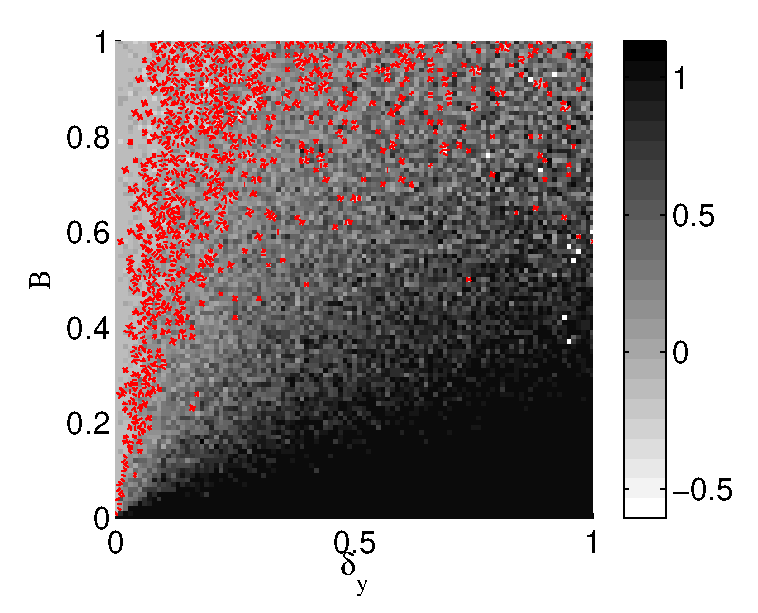
\includegraphics[scale=0.30]{SimpleIRexample_diffLpart1.eps} &
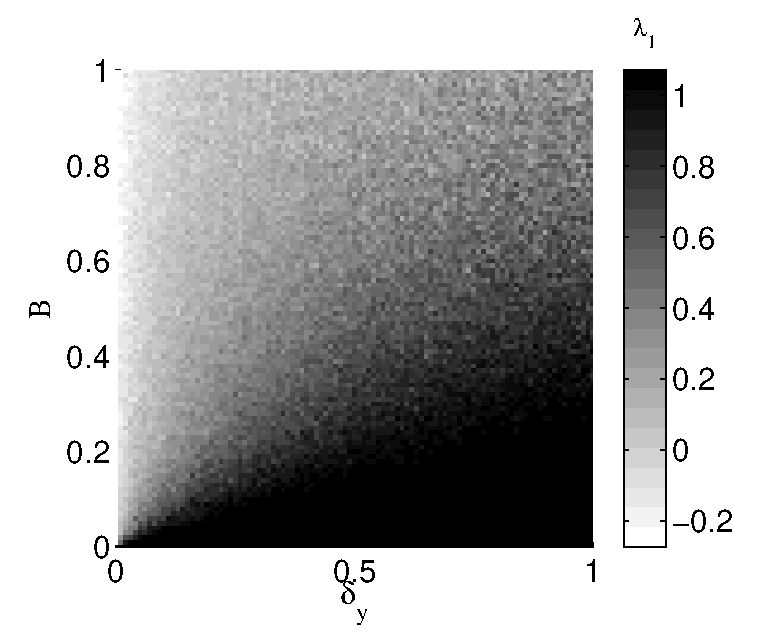
\includegraphics[scale=0.30]{SimpleIRexample_diffLpart2.eps} \\
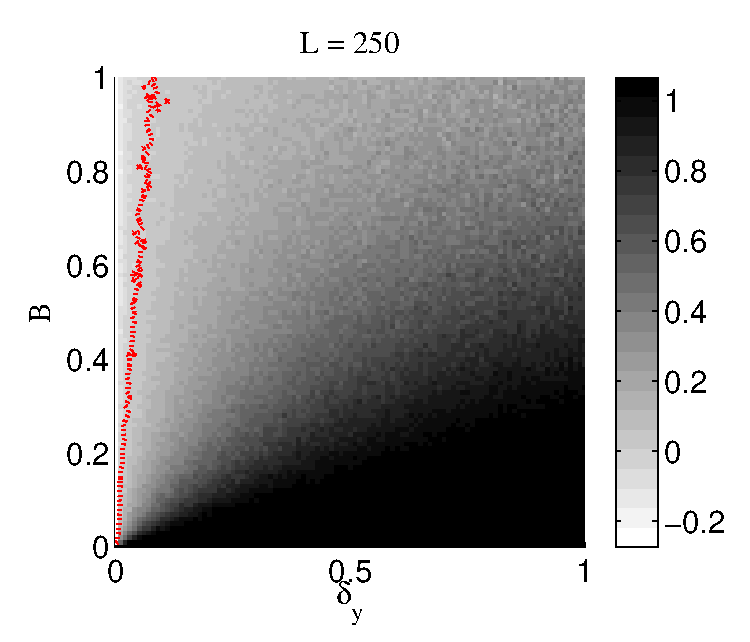
\includegraphics[scale=0.30]{SimpleIRexample_diffLpart3.eps} &
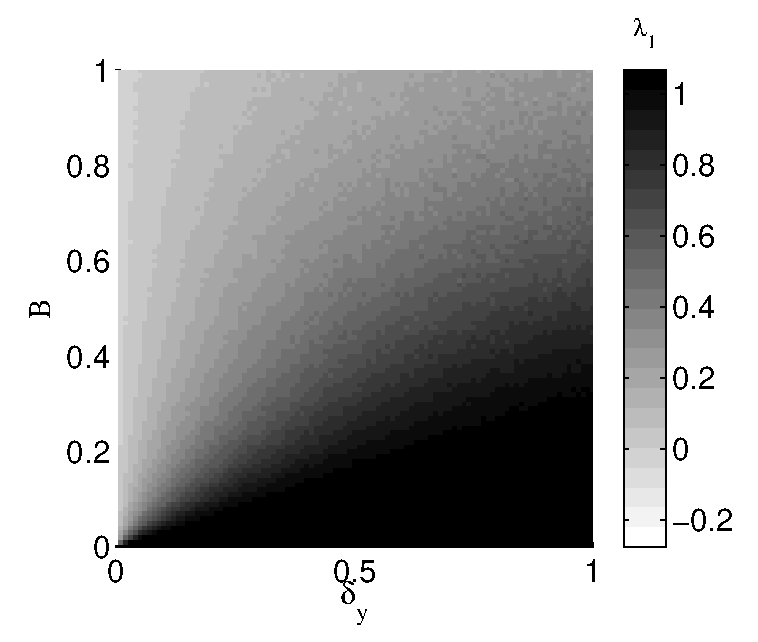
\includegraphics[scale=0.30]{SimpleIRexample_diffLpart4.eps}
\end{tabular}
\caption{(Color available online.) The unitless leaning is a function of both the noise, the tolerance used for terms from $\mathbf{Y}$, and the library length of the signals.  This synthetic data is used to explore the leaning, so $\mathbf{X}$ and $\mathbf{Y}$ do not have explicit units, from which it follows that both $\delta_y$ and $B$ are unitless.  The red dashed line is the zero contour.  See the text for am explanation of the missing data for large $\delta_y$.}
\label{fig:IRexChangeL}
\end{figure}

Figure \ref{fig:IRexChangeL} shows how the weighted mean observed leaning using the 1-standard cause-effect assignment, $\tilde{\lambda}$, changes as the noise amplitude $B$ and tolerance $\delta_y$ in increments of 0.01.  The synthetic data sets $\mathbf{X}$ and $\mathbf{Y}$ are constructed such that intuitively $\mathbf{X}$ drives $\mathbf{Y}$.  Thus, it is expected that $\mathbf{X}\xrightarrow{lean}\mathbf{Y}$ which implies $\tilde{\lambda} > 0$.  Figure \ref{fig:IRexChangeL} shows that this expectation is met except when $\delta_y < B$ even for a short library length of $L=10$.  Examples of undefined penchants due to large tolerance domains, as discussed in section \ref{sec:tol}, are seen as $\delta_y$ is increased in the $L=10$ example.

Figure \ref{fig:IRexChangeL} shows using the strategy of $\delta_y = B$ always leads to causal inferences that agree with intuition for $L>10$ in this example.  However, as discussed in section \ref{sec:tol}, knowing $B$ {\em a priori} may be unrealistic with empirical data sets.  Consider the following three methods for estimating $\delta_y$ from the data:
\begin{enumerate}
\item {\em lagged linear response deviation} - The y-tolerance is set to the mean absolute deviation of $y_t$ from $x_{t-1}$; i.e.\ $\delta_y = \langle|y_t-x_{t-1}|\rangle$.
\item {\em normalized standard deviation} - The y-tolerance is set to the standard deviation of $\{\mathbf{Y}-\langle\mathbf{Y}\rangle\}$ where $\langle\mathbf{Y}\rangle$ is the mean of $\mathbf{Y}$; i.e.\ $\delta_y = \sigma_{|y-\langle y\rangle|}$.
\item {\em n-bin mean standard deviation} - The y-tolerance is set to the mean standard deviation of $n$ bins of $\mathbf{Y}$; i.e.\ $\delta_y = \langle \sigma_{B_i}\rangle$ where $B_i$ is the $i$th bin of an $n$-bin histogram of $\mathbf{Y}$.
\end{enumerate}  

$L=100$, $B=0.5$, and $n=5$
\begin{table}
\begin{tabular}{lccc}
lag & method 1 & method 2 & method 3\\
\hline
1 & 0.39 & 0.79 & 0.18\\
2 & -0.03 & -8.0\times 10^{-5} & -0.05\\
3 & -0.38 & -0.58 & -0.33 \\
4 & -0.04 & 0 & -0.04 \\
5 &  
\end{tabular}
\caption{TBD}
\label{tab:IRlagTolComp}
\end{table}

\begin{figure}[ht]
%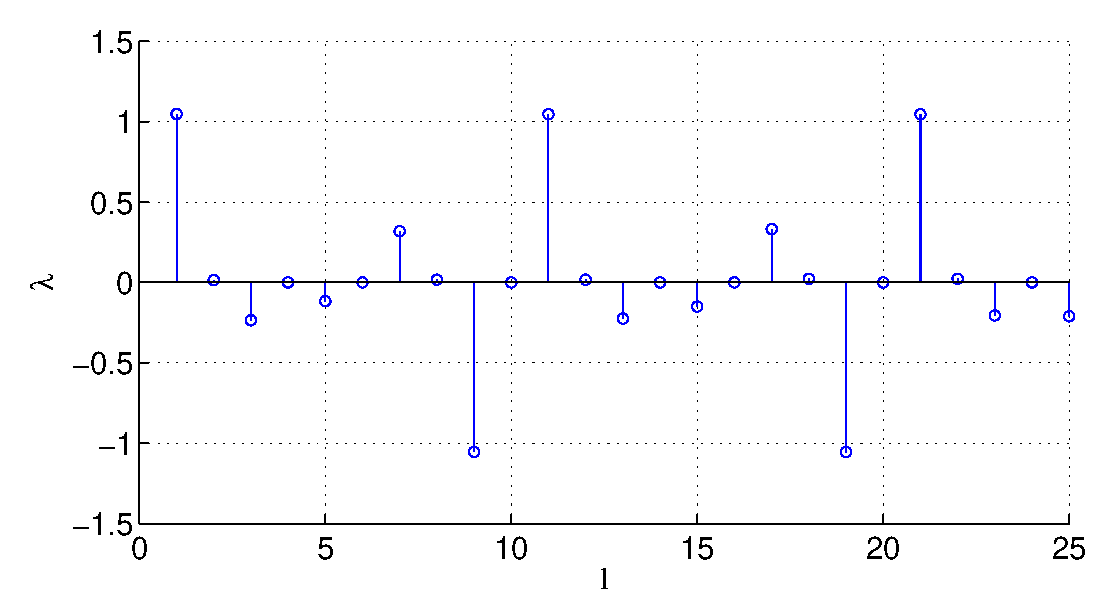
\includegraphics[scale=0.45]{SimpleIRexample_difflags.eps}
\caption{(Color available online.) Different $l$-standard cause-effect assignments lead to different leanings.}
\end{figure}

\subsection{Cyclic Linear Example}
Consider the linear example dynamical system of
\begin{eqnarray}
\label{eq:linearex}
X_t &=& \sin(t)\\
Y_t &=& X_{t-1}+B\eta_t,
\end{eqnarray}
with $B\in\mathbb{R}\ge 0$ and $\eta_t\sim\mathcal{N}\left(0,1\right)$.  Specifically, consider $B\in[0,2]$ in increments of 0.02.  The response system $Y$ is just a lagged version of the driving signal with varying levels of standard Gaussian noise applied at each time step.  
\begin{figure}[ht]
%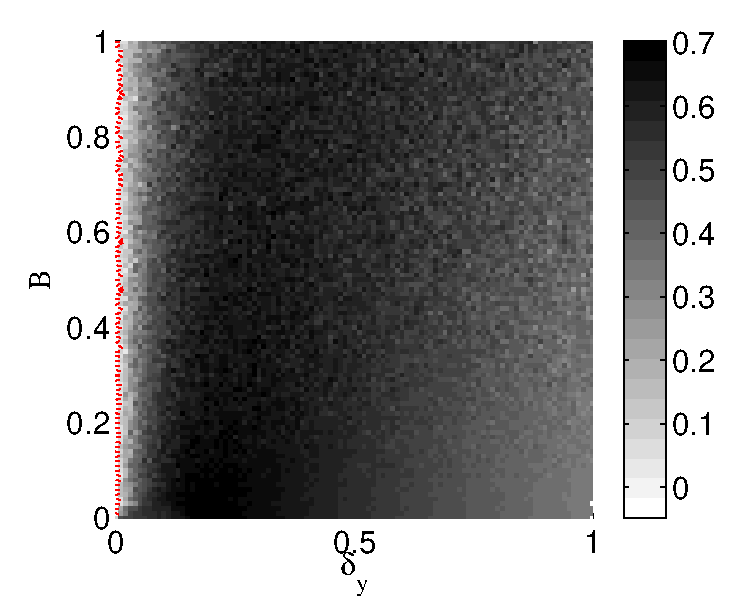
\includegraphics[scale=0.65]{SimpleCyclicexample_Bdy.eps}
\caption{(Color available online.) Leaning as a function of both the noise and the y-tolerance.  The red dashed line is the zero contour.  See the text for am explanation of the missing data for large $\delta_y$.}
\end{figure}
\begin{figure}[ht]
%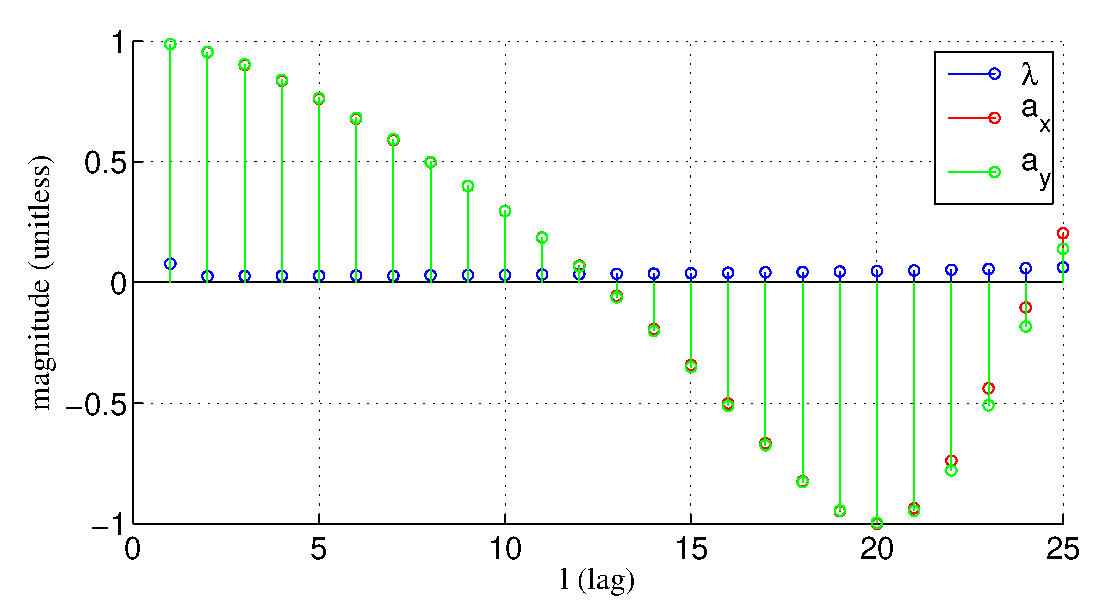
\includegraphics[scale=0.45]{SimpleCyclicexample_difflags.eps}
\caption{(Color available online.) Different $l$-standard cause-effect assignments lead to different leanings.}
\end{figure}

\subsection{Non-Linear Example}
Consider the non-linear dynamical system of
\begin{eqnarray}
\label{eqn:nonlinearEX}
X_t &=& \sin(t)\\
Y_t &=& AX_{t-1}\left(1-BX_{t-1}\right)+C\eta_t,
\end{eqnarray}
with $A,B,C\in\mathbb{R}\ge 0$ and $\eta_t\sim\mathcal{N}\left(0,1\right)$.  Specifically, consider $A,B,C\in[0,5]$ in increments of 0.5.
\begin{figure}[ht]
\begin{tabular}{cc}
%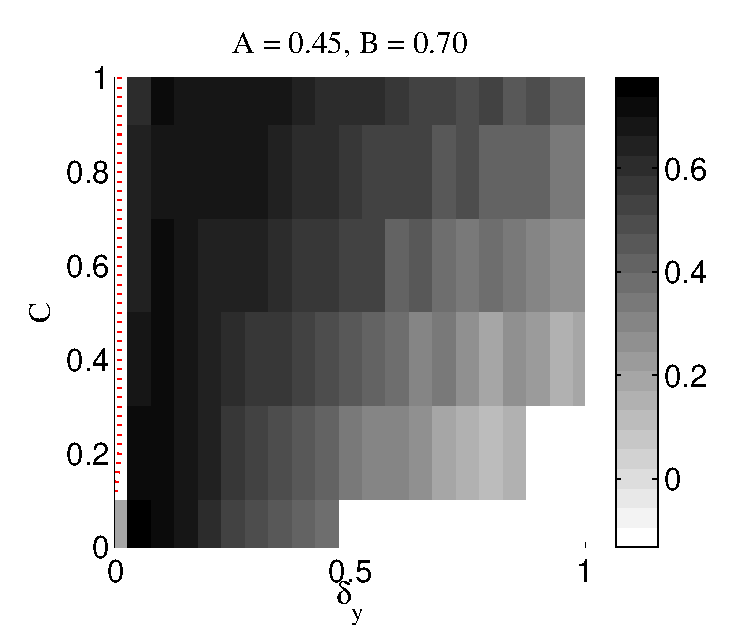
\includegraphics[scale=0.30]{NonlinearCyclicexample_Bdy_A45B70.eps} &
%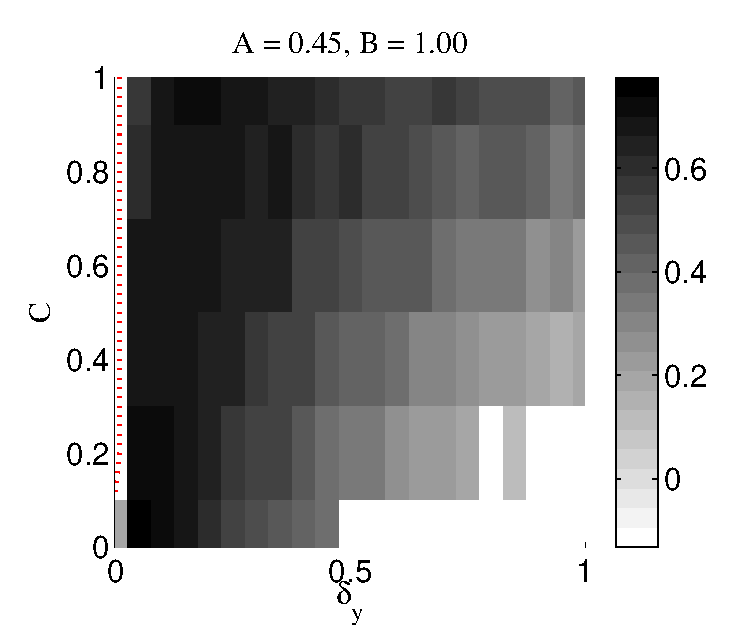
\includegraphics[scale=0.30]{NonlinearCyclicexample_Bdy_A45B100.eps} \\
%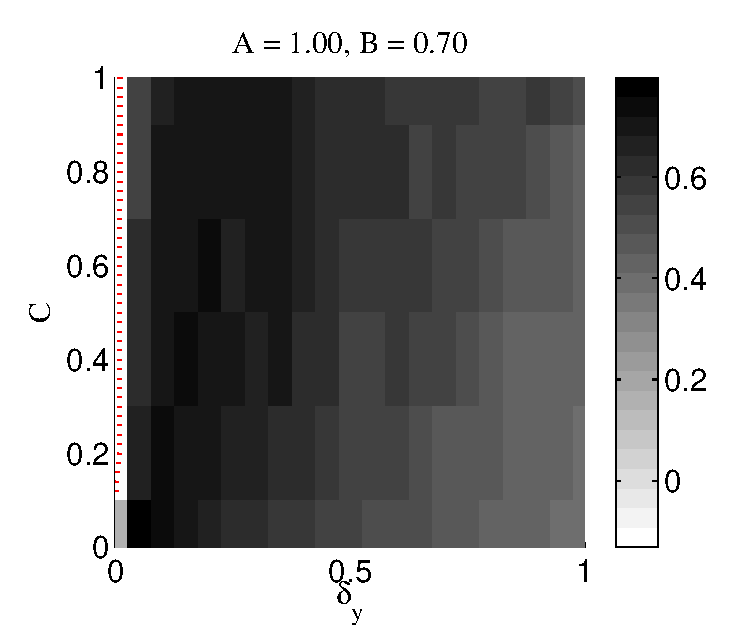
\includegraphics[scale=0.30]{NonlinearCyclicexample_Bdy_A100B70.eps} &
%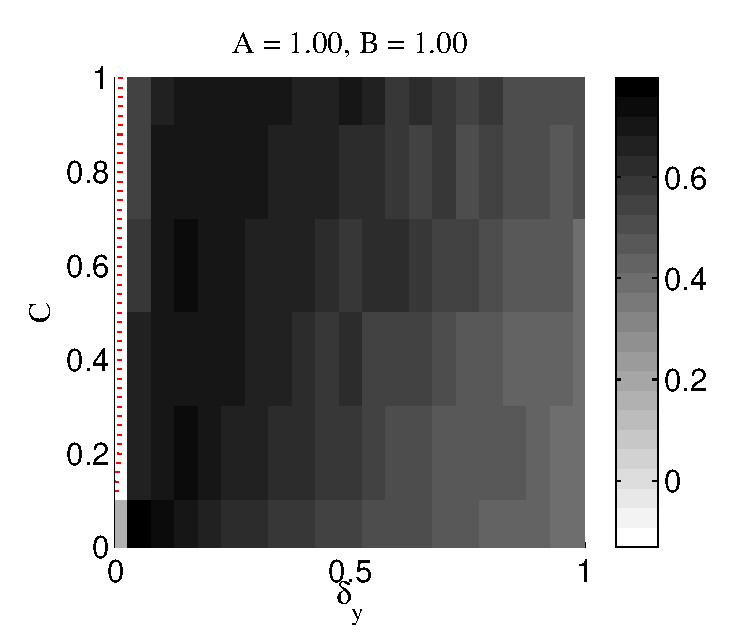
\includegraphics[scale=0.30]{NonlinearCyclicexample_Bdy_A100B100.eps} \\
\end{tabular}
\caption{(Color available online.) Leaning as a function of both the noise and the y-tolerance for values of $A$ and $B$.  The red dashed line is the zero contour.  See the text for am explanation of the missing data for large $\delta_y$.}
\end{figure}
\begin{figure}[ht]
%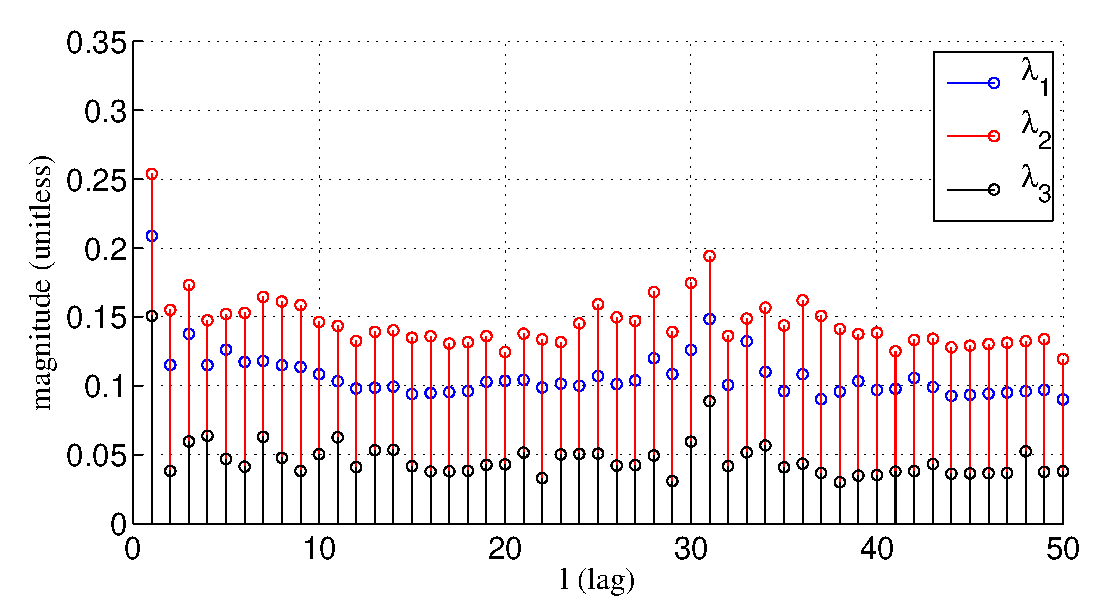
\includegraphics[scale=0.45]{NonlinearCyclicexample_difflags.eps}
\caption{(Color available online.) Different $l$-standard cause-effect assignments lead to different leanings.}
\end{figure}  

\subsection{RL Circuit Example}
\label{sec:rlcirc}
Both of the previous examples included a noise term, $\eta_t$.  Consider a series circuit containing a resistor, inductor, and time varying voltage source related by
\begin{equation}
\label{eqn:it}
\frac{dI}{dt} = \frac{V(t)}{L} - \frac{R}{L} I,
\end{equation}
where $I$ is the current at time $t$, $V(t)= \sin\left(\Omega t\right)$ is the voltage at time $t$, $R$ is the resistance, and $L$ is the inductance.  Eqn. \ref{eqn:it} was solved using the {\em ode45} integration function in MATLAB.  The time series $V(t)$ is created by defining values at fixed points and using linear interpolation to find the time steps required by the ODE solver.  

Consider the situation where $L=10$ Henries and $R=5$ Ohms are constant.  Physical intuition is that $V$ drives $I$, and so we expect to find that $V$ CCM causes $I$ (i.e., $C_{VI}>C_{IV}$ or $\Delta = C_{VI}-C_{IV} > 0$). 
\begin{equation}
I = \frac{L}{D}e^{-\frac{R}{L}t}+\frac{R}{D}\sin(t)-\frac{L}{D}\cos(t)
\end{equation}
with $D = L^2 + R^2$.   


\subsection{Impulse with Multiple Noisy Responses Example}
\begin{eqnarray}
\bar{\mathbf{\tau}}_L = \left\{\mathbf{X},\mathbf{Y},\mathbf{Z}\right\} = \left\{\{x_t\},\{y_t\},\{z_t\}\right\}
\end{eqnarray}
where $t\in[0,L]$,
\begin{equation*}
x_t = \left\{
  \begin{array}{lr}
    2 & t = 1\\
    0 & \forall\; t\in\{t\;|\;t\neq 1 \;\mathrm{and}\; t\bmod 5 \neq 0\}\\
    2 & \forall\; t\in\{t\;|\;t\bmod 5 = 0\}
  \end{array}
\right.
\end{equation*}
\begin{eqnarray*}
y_t &=& x_{t-1} + B\eta_t\\
z_t &=& y_{t-1}\\
z_t^\prime &=& y_{t-1} + y_t = y_{t-1} + x_{t-1} + B\eta_t\\
z_t^{\prime\prime} &=& y_{t-1} + x_{t-1} + z_{t-1}
\end{eqnarray*}
with $y_0 = 0$, $B\in\mathbb{R}\ge 0$, $\eta_t\sim\mathcal{N}\left(0,1\right)$, and $L=500$.
\begin{figure}[ht]
%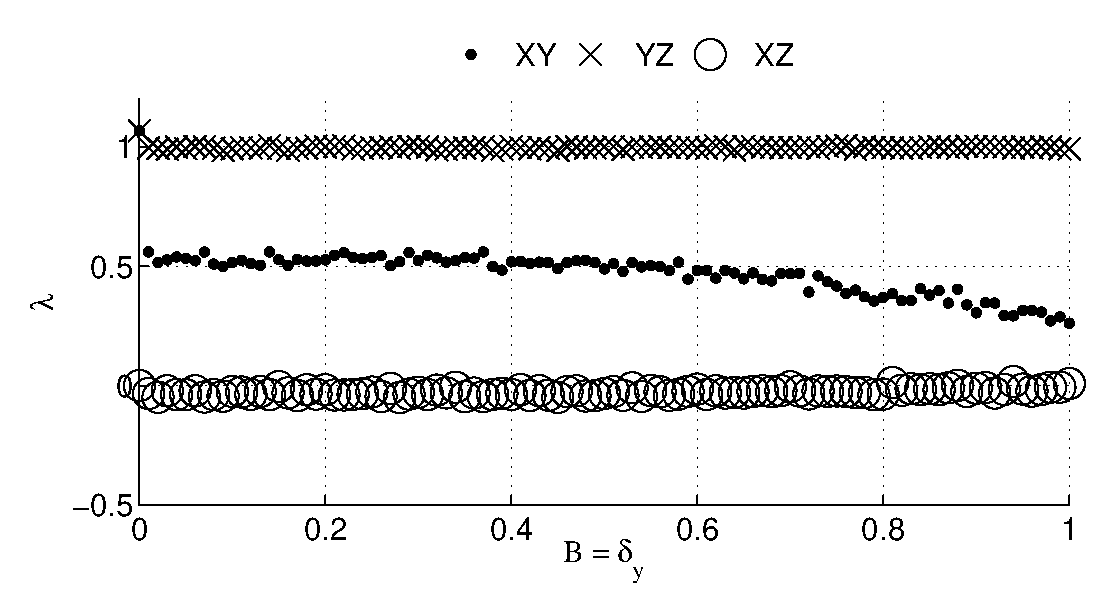
\includegraphics[scale=0.45]{XYZIRexample_Bxytol.eps}
\caption{$\left\{\mathbf{X},\mathbf{Y},\mathbf{Z}\right\}$}
\end{figure}
\begin{figure}[ht]
%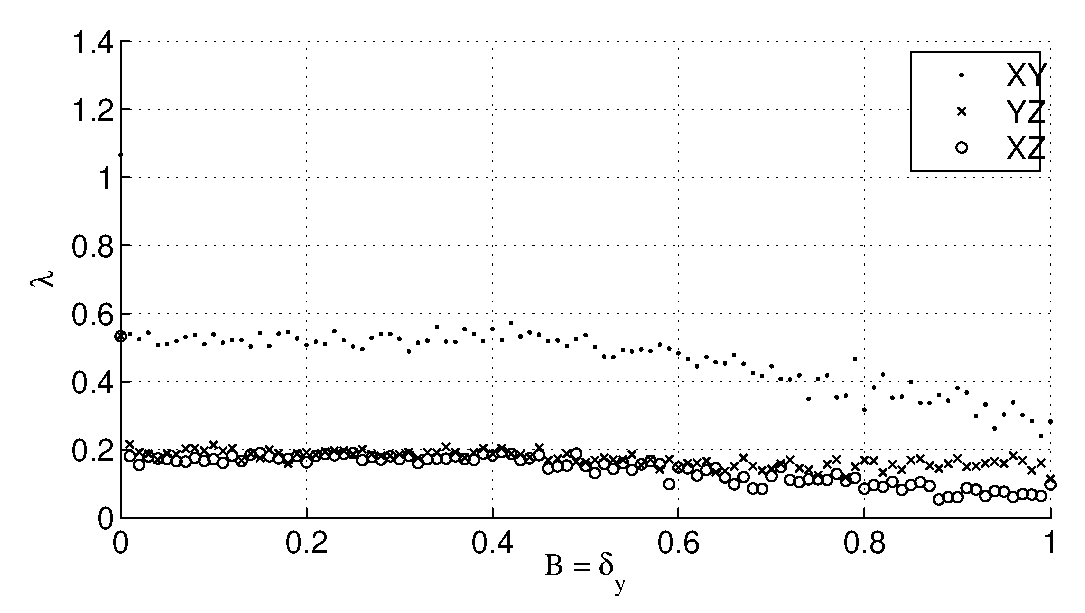
\includegraphics[scale=0.45]{XYZIRexample_BxytolZXandY.eps}
\caption{$\left\{\mathbf{X},\mathbf{Y},\mathbf{Z}^\prime\right\}$}
\end{figure}
\begin{figure}[ht]
%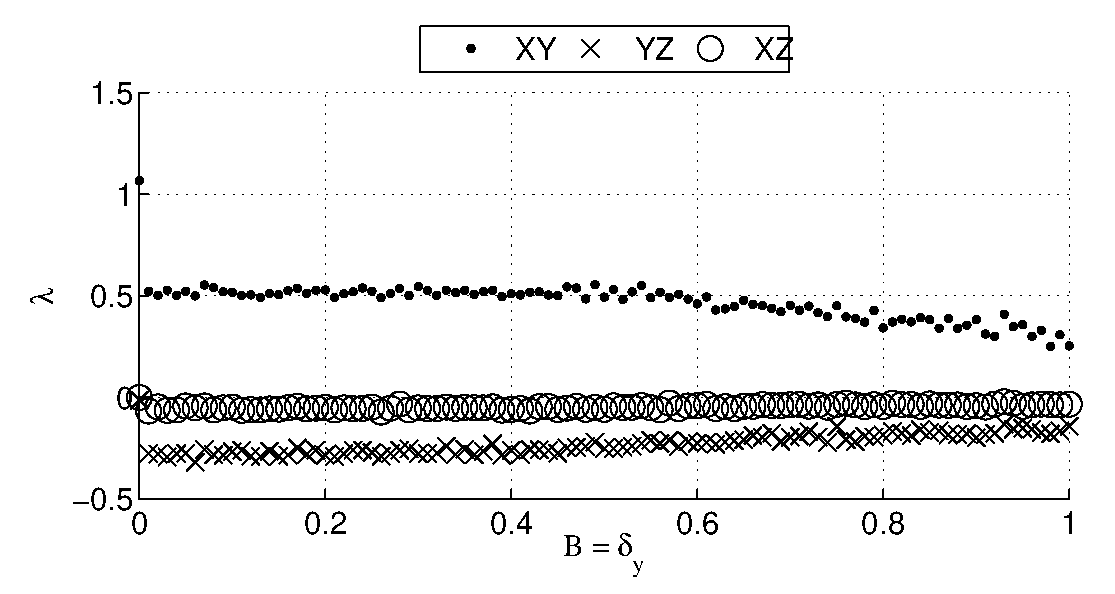
\includegraphics[scale=0.45]{XYZIRexample_BxytolZXandYandZ.eps}
\caption{$\left\{\mathbf{X},\mathbf{Y},\mathbf{Z}^{\prime\prime}\right\}$}
\end{figure}

\section{Empirical Data}

\section{Conclusion}

%\bibliographystyle{plain}
%\bibliography{main}

\end{document}